\documentclass{beamer}
\usetheme{metropolis}           % Use metropolis theme
\title{Exploring the role of rewiring on the structure of ecological interaction networks:\newline a simulation-based approach}
\date{July 5, 2024}
\author{Rémi Legrand}
\institute{Laboratoire de Biometrie et Biologie Évolutive}

\begin{document}

\maketitle

\begin{frame}{Importance of predicting interactions in a changing environment}

  \begin{columns}
    \begin{column}{.3\linewidth}
      \includegraphics<1->[width=\linewidth]{figures_slides/biodiv_loss_giec.png}
    \end{column}
    \begin{column}{.7\linewidth}
      \includegraphics<2>[width=\linewidth]{figures_slides/temperature_raising.pdf}
    \end{column}
  \end{columns}
  \vfill
  {\scriptsize \uncover<1->{IPBES report 2019} \hfill \uncover<2->{IPCC report v5 2023}}
\end{frame}

\begin{frame}{Factors to predict interactions}

  \begin{columns}
    \begin{column}{.4\linewidth}
      %\only<3>{Salut}
      %\uncover<3>{Salut}
      \begin{itemize}
      \item<1-> \textbf{Abundances}
      \item<2-> \textbf{Trait matching} %% The influence of biogeographical and evolutionary
        %% histories on morphological trait-matching and resource specialization
        %% in mutualistic hummingbird--plant networks
      \item<3-> \textbf{Phenology}
      \item<4-> \textbf{Others}  adaptation capability (rewiring)
      \end{itemize}
    \end{column}
    \begin{column}{.6\linewidth}
      \includegraphics<1>[width=\linewidth]{figures_slides/abundance.png}%
      \includegraphics<2>[width=\linewidth]{figures_slides/trait_matching.png}%
      \includegraphics<3>[width=\linewidth]{figures_slides/phenology.png}%
      \includegraphics<4>[width=\linewidth]{figures_slides/other_rewiring.png}%
    \end{column}
  \end{columns}
\end{frame}

\section{Exploring the role of rewiring on the structure of ecological interaction networks:\newline a simulation-based approach}


\begin{frame}{Current method to compute rewiring: Beta diversity}
\protect\hypertarget{current-method-to-compute-rewiring}{}
\begin{columns}
  \begin{column}{.5\linewidth}
    \uncover<1->{$$\beta_{dissimilarity} = \frac{|a|+|c|+|b|}{\frac{|a|}{2} + |c|+ \frac{|b|}{2}} - 1$$}
    \uncover<2->{$$\beta_{WN} = \beta_{ST} + \beta_{OS}$$}\vspace{-1em}
    \uncover<3->{$$\Delta\beta_{OS,i} = \beta_{OS} - \beta_{OS,\Delta i}$$}
  \end{column}
  \begin{column}{.5\linewidth}
    \includegraphics<1->[width=\linewidth]{figures_slides/beta_div.png}%
  \end{column}
\end{columns}
\end{frame}

\begin{frame}{How do we plan to study rewiring : CA}
\protect\hypertarget{How-do-we-plan-to-study-rewiring-:-CA}{}
\begin{columns}
  \begin{column}{.5\linewidth}
    \includegraphics<1->[width=\linewidth]{figures_slides/network.png}%
  \end{column}
  \begin{column}{.5\linewidth}
    \includegraphics<2->[width=\linewidth]{figures_slides/AFC.png}%
  \end{column}
\end{columns}
\end{frame}
\begin{frame}{Multinetwork extension: Foucart CA}
\protect\hypertarget{foucart-ca}{}
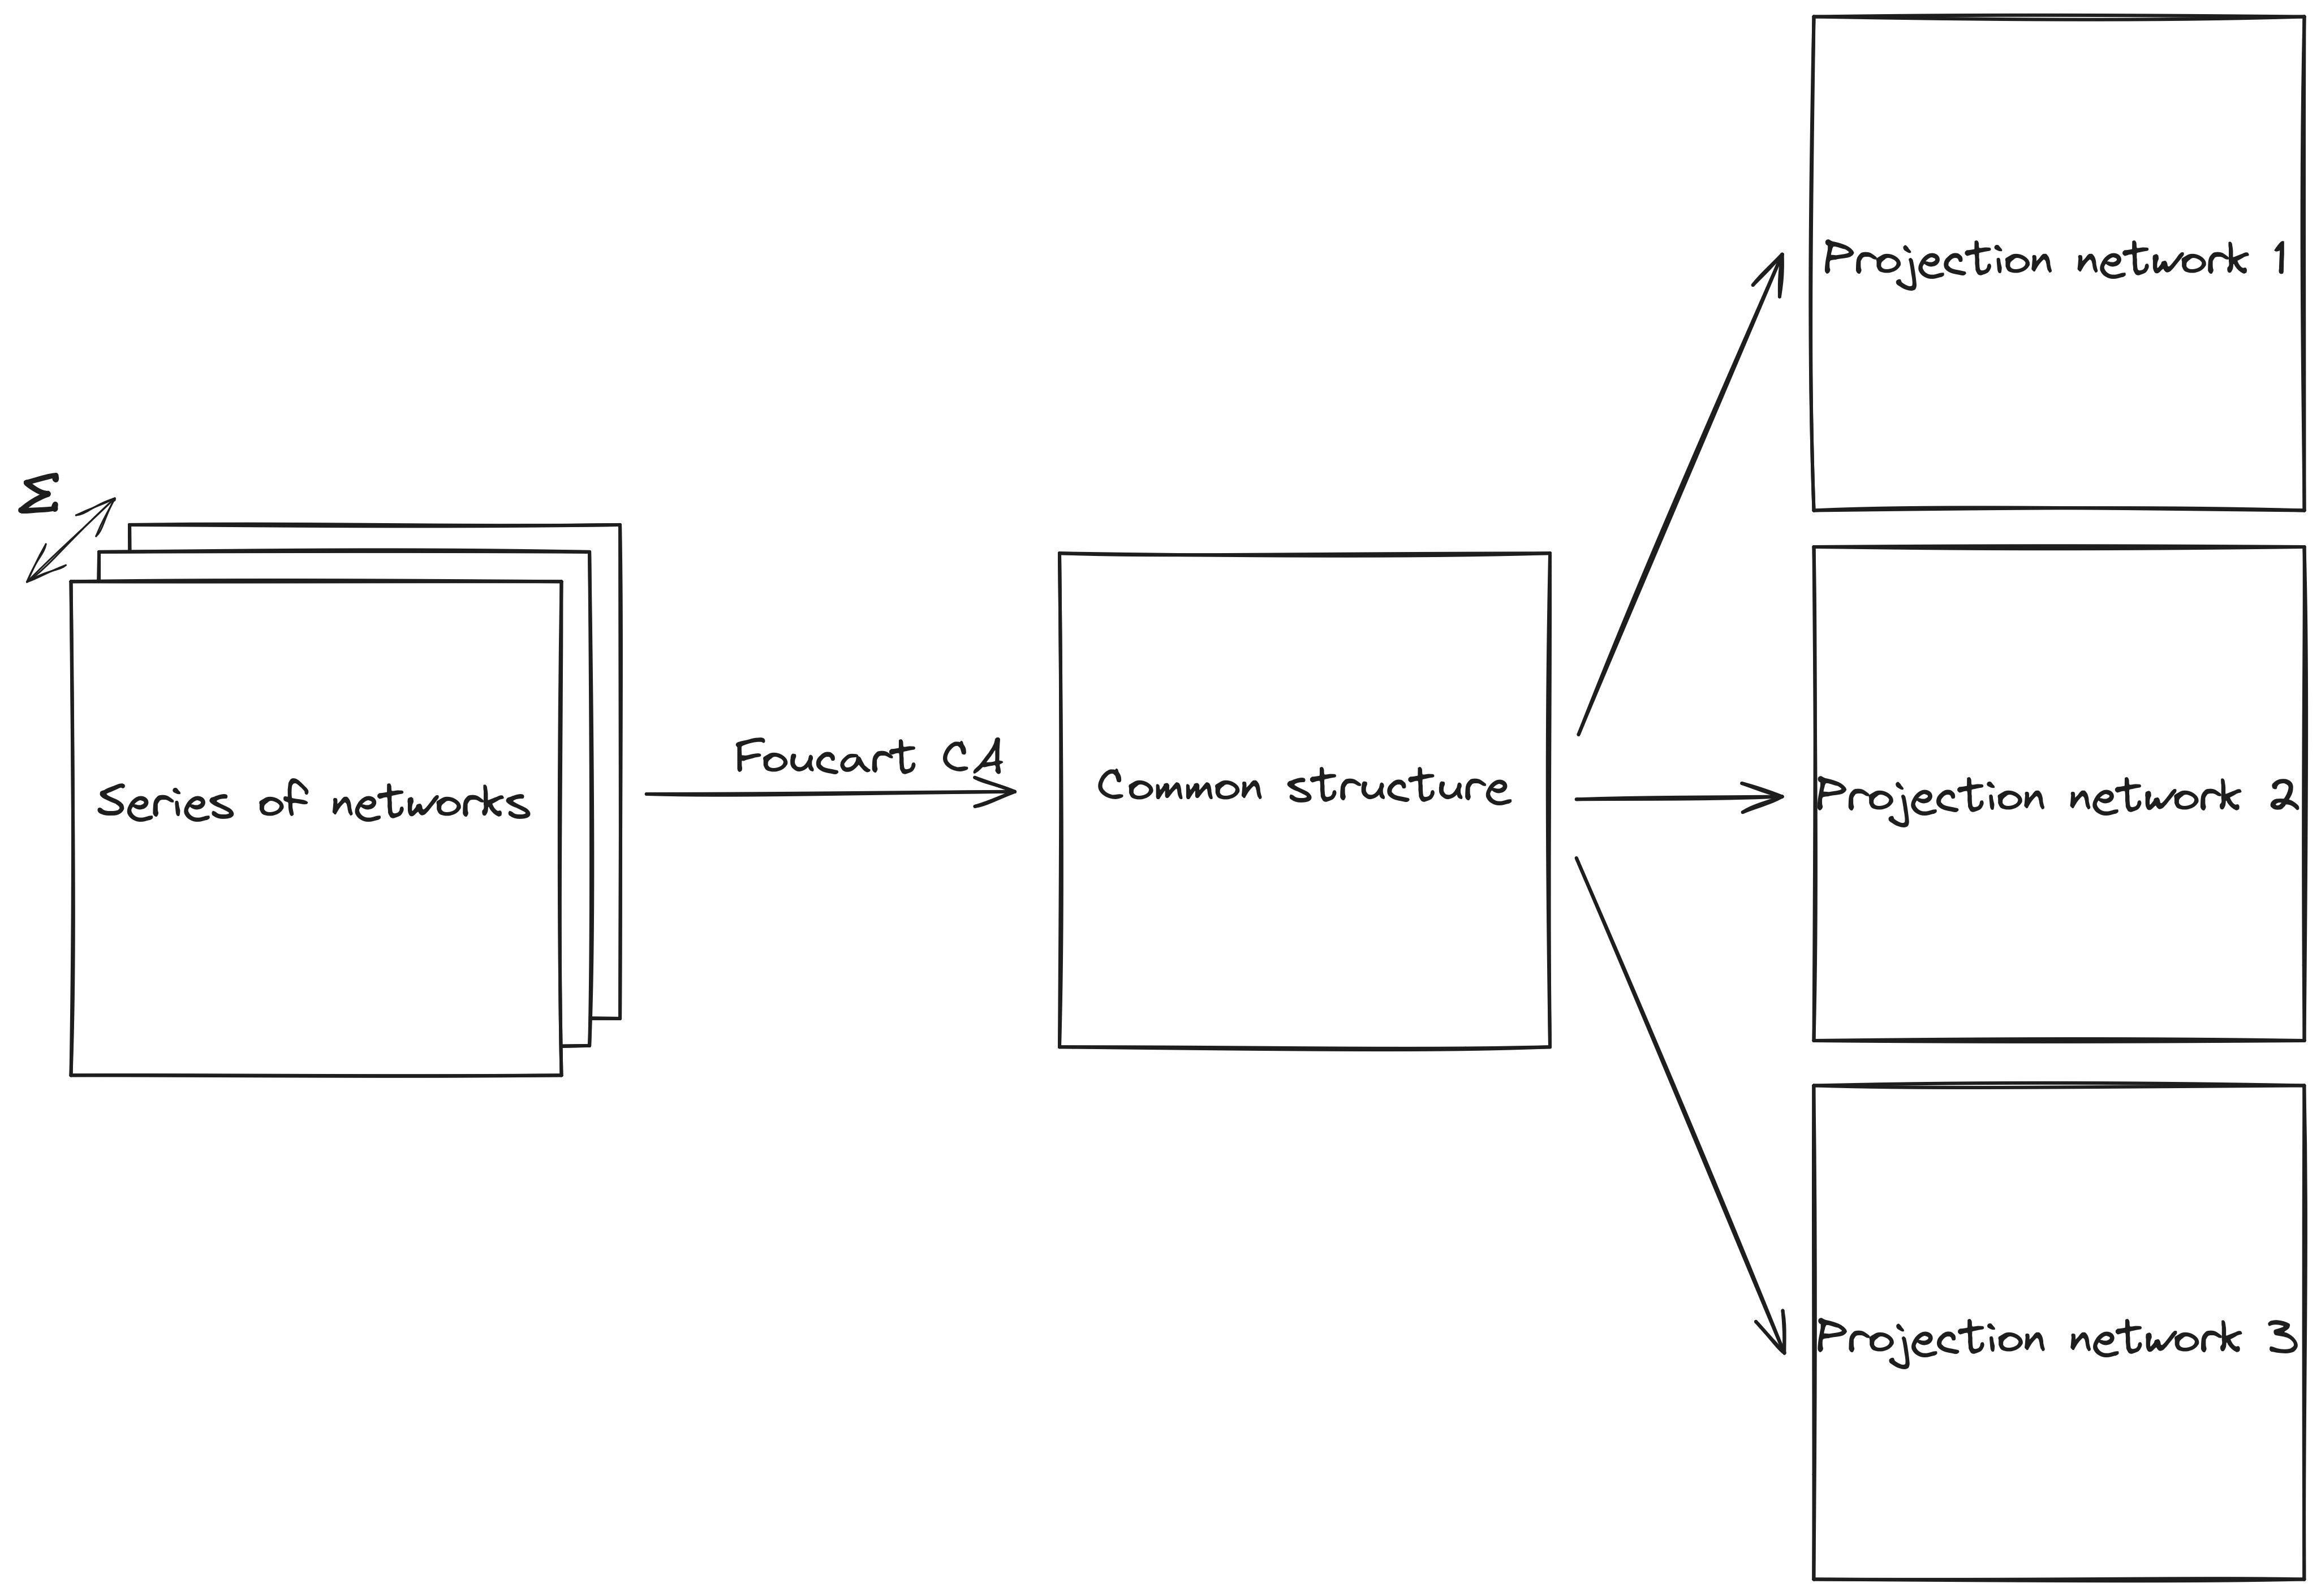
\includegraphics[width=\linewidth]{figures_slides/foucart.png}%
\end{frame}

\begin{frame}{Compare to other methods}
  \framesubtitle{(or did it?)}
  \begin{columns}
    \begin{column}{.5\linewidth}
      \includegraphics<1->[width=\linewidth]{figures_slides/rewiring.pdf}%
    \end{column}
    \begin{column}{.5\linewidth}
      \begin{minipage}{\linewidth}
        \includegraphics<2->[width=\linewidth]{figures_slides/impact_env.pdf}\\ [1cm]
        \includegraphics<2->[width=\linewidth]{figures_slides/impact_trait_tol.pdf}%
      \end{minipage}
    \end{column}
  \end{columns}
\end{frame}


\begin{frame}{Why it did not work?}
  \begin{columns}
    \begin{column}{.5\linewidth}
      \includegraphics<1->[width=\linewidth]{figures_slides/simulation_limits.png}%
    \end{column}
    \begin{column}{.5\linewidth}
      \includegraphics<2->[width=\linewidth]{figures_slides/foucart_limits.png}%
    \end{column}
  \end{columns}
\end{frame}

\begin{frame}{Perspectives}
\protect\hypertarget{perspectives}{}
\begin{itemize}
\item
  Improve the Beta dissimilarity computation
\item
  Correct the simulation bias
\end{itemize}
\end{frame}

\section*{Thanks for your attention!}

\begin{frame}{Simulation process}
  \centering
  \includegraphics<1->[height=0.95\textheight, keepaspectratio]{figures_slides/Netw_generation.png}%
\end{frame}

\begin{frame}{Trait recovery}
  \includegraphics<1->[width=\linewidth]{figures_slides/supplements/ninter.pdf}%
\end{frame}

\begin{frame}{Trait recovery}
  \includegraphics<1->[width=\linewidth]{figures_slides/supplements/frame_env.pdf}%
\end{frame}

\begin{frame}{Trait recovery}
  \includegraphics<1->[width=\linewidth]{figures_slides/supplements/delta.pdf}%
\end{frame}

\begin{frame}{Trait recovery}
  \includegraphics<1->[width=\linewidth]{figures_slides/supplements/ratio.pdf}%
\end{frame}

\begin{frame}{Trait recovery}
  \includegraphics<1->[width=\linewidth]{figures_slides/supplements/trait.pdf}%
\end{frame}


\end{document}
